% Options for packages loaded elsewhere
\PassOptionsToPackage{unicode}{hyperref}
\PassOptionsToPackage{hyphens}{url}
%
\documentclass[
]{book}
\usepackage{amsmath,amssymb}
\usepackage{lmodern}
\usepackage{ifxetex,ifluatex}
\ifnum 0\ifxetex 1\fi\ifluatex 1\fi=0 % if pdftex
  \usepackage[T1]{fontenc}
  \usepackage[utf8]{inputenc}
  \usepackage{textcomp} % provide euro and other symbols
\else % if luatex or xetex
  \usepackage{unicode-math}
  \defaultfontfeatures{Scale=MatchLowercase}
  \defaultfontfeatures[\rmfamily]{Ligatures=TeX,Scale=1}
\fi
% Use upquote if available, for straight quotes in verbatim environments
\IfFileExists{upquote.sty}{\usepackage{upquote}}{}
\IfFileExists{microtype.sty}{% use microtype if available
  \usepackage[]{microtype}
  \UseMicrotypeSet[protrusion]{basicmath} % disable protrusion for tt fonts
}{}
\makeatletter
\@ifundefined{KOMAClassName}{% if non-KOMA class
  \IfFileExists{parskip.sty}{%
    \usepackage{parskip}
  }{% else
    \setlength{\parindent}{0pt}
    \setlength{\parskip}{6pt plus 2pt minus 1pt}}
}{% if KOMA class
  \KOMAoptions{parskip=half}}
\makeatother
\usepackage{xcolor}
\IfFileExists{xurl.sty}{\usepackage{xurl}}{} % add URL line breaks if available
\IfFileExists{bookmark.sty}{\usepackage{bookmark}}{\usepackage{hyperref}}
\hypersetup{
  pdftitle={Dementia research under a causal inference lens},
  pdfauthor={Liliana Paloma Rojas Saunero},
  hidelinks,
  pdfcreator={LaTeX via pandoc}}
\urlstyle{same} % disable monospaced font for URLs
\usepackage{longtable,booktabs,array}
\usepackage{calc} % for calculating minipage widths
% Correct order of tables after \paragraph or \subparagraph
\usepackage{etoolbox}
\makeatletter
\patchcmd\longtable{\par}{\if@noskipsec\mbox{}\fi\par}{}{}
\makeatother
% Allow footnotes in longtable head/foot
\IfFileExists{footnotehyper.sty}{\usepackage{footnotehyper}}{\usepackage{footnote}}
\makesavenoteenv{longtable}
\usepackage{graphicx}
\makeatletter
\def\maxwidth{\ifdim\Gin@nat@width>\linewidth\linewidth\else\Gin@nat@width\fi}
\def\maxheight{\ifdim\Gin@nat@height>\textheight\textheight\else\Gin@nat@height\fi}
\makeatother
% Scale images if necessary, so that they will not overflow the page
% margins by default, and it is still possible to overwrite the defaults
% using explicit options in \includegraphics[width, height, ...]{}
\setkeys{Gin}{width=\maxwidth,height=\maxheight,keepaspectratio}
% Set default figure placement to htbp
\makeatletter
\def\fps@figure{htbp}
\makeatother
\setlength{\emergencystretch}{3em} % prevent overfull lines
\providecommand{\tightlist}{%
  \setlength{\itemsep}{0pt}\setlength{\parskip}{0pt}}
\setcounter{secnumdepth}{5}
\usepackage{booktabs}
\ifluatex
  \usepackage{selnolig}  % disable illegal ligatures
\fi
\usepackage[style=apa,]{biblatex}
\addbibresource{book.bib}
\addbibresource{packages.bib}

\title{Dementia research under a causal inference lens}
\author{Liliana Paloma Rojas Saunero}
\date{2021-08-26}

\begin{document}
\maketitle

{
\setcounter{tocdepth}{1}
\tableofcontents
}
Testing

\hypertarget{intro}{%
\chapter{Introduction}\label{intro}}

\hypertarget{the-burden-of-alzheimers-disease-and-dementia}{%
\section{The burden of Alzheimer's disease and dementia}\label{the-burden-of-alzheimers-disease-and-dementia}}

With extension of life expectancy over the last few decades, Dementia has become a major burden that affects the elderly. In 2016, the global number of individuals who lived with dementia was over 40 \autocite{gbd2016} million and by 2050 this number is expected to triplicate \autocite{worldreport2018}. In 2020, deaths due to Alzheimer's disease and other dementias have increased, becoming the 7th leading cause of death globally and overtaking stroke to become the second leading cause in high-income countries\autocite{who2020}. Women are disproportionately affected, accounting for 65\% of deaths from dementia. Furthermore, the risk of dementia among populations from Low-middle income countries is increasing steeply, and it affects Latino, Black and other minorities disproportionately, worldwide. The burden of dementia does not only affect those who have the disease, it largely affect the lives of those who act as caregivers, families, and health-care systems. It may have sever repercussions, specially in poor and marginalized areas, given that the burden of caregiving disproportionately affects women. Unequal distribution of opportunities and responsibilities and societal roles may push women into the caregiver role more than men, which hampers even more their access to paid work and health, creating negative feedback loops that increases all kinds of disparities \autocite[\textcite{brodaty2009}, \textcite{etters2008}]{swinkels2019}.

Given that dementia is a complex and heterogeneous disease, with multiple etiologic and neuropathologic processes related, there is an urge to identify modifiable risk factors and therapies that both prevent and delay the onset of dementia, as well as slow progression and reduce symptoms of disease. To this purpose, in 2020, the Lancet Commision released an updated guideline with evidence on twelve modifiable risks factors, which would account for 40\% of worldwide dementias that could have been prevented or delayed \autocite{dementia_lancet}. These modifiable risk factors include: less education, hypertension, hearing impairment, smoking, obesity, depression, physical inactivity, diabetes, low social contact, alcohol consumption, traumatic brain injury (TBI), and air pollution.

A growth for biomarker/ biological mechanisms research, which serves as proxy for dementia, but that could act as targets for intervention.

In respect to therapies, there are few specific drugs that target amyloid and thau production, though with small evidence. Thus, new studies for drugs that target other mechanismis are in study. There is a call for drug repositioning and repurposing, which may offer a valuable alternative route for the identification of effective disease-modifying treatments for dementia. Drug repurposing, meaning the application of established drug compounds to new therapeutic indications \autocite[\textcite{langedijk2015}]{ballard2020}. In 2020, Cummiengs et al.~identified 121 agents in clinical trials for the treatment of Alzheimer's disease, out of which 43\% (57) represented repurposed agents across all phases of the pipeline \autocite{cummings2020}. Furthermore, approaches to identify potential drugs are often based on observational studies, as the use of large datasets to detect drug-associated patient outcomes becomes more available.

\hypertarget{giving-causal-inference-a-second-chance}{%
\section{Giving causal inference a second chance}\label{giving-causal-inference-a-second-chance}}

Observational studies have been essential to move forward in the understanding of the disease and current availability of multiple sources of large data give us the opportunity to expand the field. Nevertheless, the availability of data sources and sophisticated computational software may sometimes overshadow the process of asking clear questions and the steps to tie the causal questions to the data. But acknowledging that etiologic research in dementia research represents causal thinking, is probably the first challenge and impediment to conceptualize a clear question. In a time were we have deeply embraced that ``causation is not correlation'', the concept of ``associations'' and training towards defining questions as hypothesis testing, has deeply overshadowed the critical step in research to clearly define questions and wanted interpretations. Likewise, extensive debates among causal inference researchers, on whether exposures that cannot be intervened up or manipulated (such as sex, race or BMI) can be framed causal questions, can be overwhelming and confusing to novice students who are trying to embrace causal thinking. At least, this was the case for me on the early years of my PhD trajectory.

Without falling into one side of the polarized debate of what is causal or not, this dissertation provides an optic to dementia etiologic research from a causal inference lens. Throughout the next chapters I will conceive all kinds of time-varying exposures such as medication treatments as in Chapter \ref{chapter2} or molecular pathways that are yet unobserved as in Chapter \ref{chapter4}, as potential targets of intervention. I will develop how the creative process of thinking and imagining what is what we truly want to ask helps to formulate clear questions, identify potential sources of bias, and articulate the analytic methods to match the question. Furthermore, I will show how this process will enhance the transparency of the research intentions, and discuss the challenges that rise regarding \emph{consistency}, one of the identifiability assumptions on causal inference. To this matter, throughout this dissertation I will embrace and implement the target trial emulation framework\autocite{labrecque2018}.

\hypertarget{target-trial-emulation-and-well-defined-interventions}{%
\section{Target trial emulation and well-defined interventions}\label{target-trial-emulation-and-well-defined-interventions}}

Since observational studies are often performed using data that was not collected specifically to answer one but rather several questions of interest, we must be cautious on the study design and analytic decisions to answear each question. The target trial emulation is the application of design principles from randomized trials to the analysis of observational data, explicitly tying the analysis to the trial it is emulating. This includes specifying the eligibility criteria, treatment strategies, treatment assignment, follow-up period, outcome, causal contrasts and statistical analysis\autocite{labrecque2018}. Describing each of these elements can be a challenging process, since there is no right or wrong. The refinement of the causal question will often be a back and forward process between the question we truly aim to answer and the availability of data to answer that question.

To illustrate how the target trial improves observational studies, in @(chapter 2) I conceptualize a target trial to study the effect of statins treatment in the 10-year risk of dementia and death. This work brings clarity to the idea that even in observational studies we can formulate causal contrasts like the intention-to-treat effect (ITT) and to the per-protocol effect (PP), as in pragmatic trials. In this setting, the intention-to-treat effect refers to a combination of the effect of the treatment under study and of any other patient and physician's behavioral changes triggered by the assignment itself, and is agnostic of any treatment decisions made after baseline, which makes it difficult to interpret to patients, clinicians and other decision-makers (\textcite{murray2019}). Thought this is what makes it appealing from an analytic perspective, since it can be conceptualized as a point treatment strategy. Instead, the per-protocol effect represents the effect of being assigned and adhere to the assigned treatment strategy through-out follow-up, as specified in the study protocol.

Furthermore, the per-protocol effect can be conceptualized as a dynamic treatment strategy, since adherence to a treatment strategy over follow-up will depend on the evolution of an individual's time-varying covariates. For example, in the case of statins, an individual can be assigned to not take statin therapy during the study, unless LDL-cholesterol is high or coronary heart disease is diagnosed. Likewise, an individual should be allowed to stop statin therapy if side effects arise. Being explicit about the treatment strategy emphasizes on the necessity to collect data on the treatment adherence over follow-up, as well as time-varying confounders and predictors of adherence. It also introduces the major challenge with time-varying treatments, the time-varying confounding feedback.

Time-varying confounding feedback refers to the setting where, time-varying covariates at time \(t\) affect treatment at time \(t\), but additionally, time-varying covariates at time \(t\) are affected themselves by treatment at time \(t - 1\).



\begin{figure}

{\centering 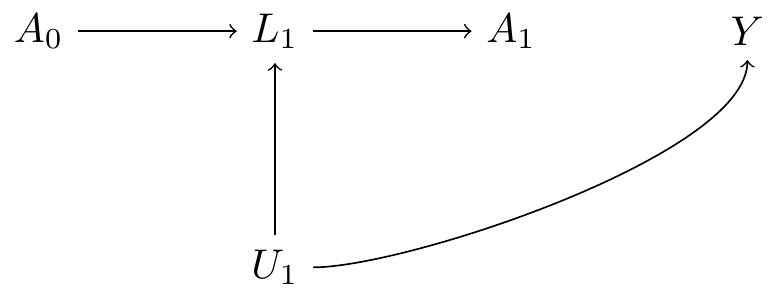
\includegraphics{thesis_bookdown_files/figure-latex/fig1-1} 

}

\caption{DAGs representing an MR study with one genetic variant \emph{Z}, proposed as an instrument for the effect of \emph{X} on \emph{Y}. In \textbf{A}, \emph{Z} is a valid instrument. In \textbf{B}, the MR assumptions are violated by a direct effect of \emph{Z} on \emph{Y}.}\label{fig:fig1}
\end{figure}

Just as we are interested in the time-varying effect of medication strategies in the risk of dementia, most of the ``risk factors'' proposed by the Lancet Comission, can be conceptualized within a target trial framework. This step would help us clarify what are the underlying interventions to be framed around these modifiable risks factors. In Chapter 3

\hypertarget{study-setting}{%
\section{Study setting}\label{study-setting}}

For this reason, in chapter 2. we begin by conceptualizing questions around the competing event of death. We
In chapter 3. we study the effect of statins in the risk of dementia. In chapter 4 we study the potential effect of interventions that reduce systolic blood pressure over time. In chapter 5 I unveil the issues around a cancer onset as an exposure, and outline the causal question behind the inverse association between cancer and dementia.

\hypertarget{aims}{%
\section{Aims}\label{aims}}

``to search for all the refutable consequences of a hypothesis demands highly imaginative thinking. Imagination is needed to arrive at the hypothesis in the first place, let alone to suggest rigorious tests for it. Although imaginative thinking is commonly regarded as an inborn ability which cannot be taught, de Bono suggests many techniques for enhancing whatever abilities a person has received from nature. (de Bono, Lateral Thinking)''

\hypertarget{dementia-diagnosis-and-death}{%
\section{Dementia diagnosis and death}\label{dementia-diagnosis-and-death}}

\begin{itemize}
\tightlist
\item
  Talk a bit about competing events, the fuzzyness around questions and unclear interpretations.
\end{itemize}

``Productive habits of thought might be acquired if thought were given more emphasis and action less'' \autocite{buck2017}

\newpage

\hypertarget{chapter2}{%
\chapter{Emulating a target trial of statin use and risk of dementia using cohort data}\label{chapter2}}

\chaptermark{Statins use and dementia risk}

\newpage

\hypertarget{abstract}{%
\section{Abstract}\label{abstract}}

\textbf{Objective:} Observational data can be used to attempt to emulate a target trial of statin use and estimate analogues of intention-to-treat and per-protocol effects on dementia risk.

\textbf{Methods:} Using data from a prospective cohort study in the Netherlands, we conceptualized a sequence of ``trials'' in which eligible individuals ages 55-80 years were classified as statin initiators or non-initiators for every consecutive month between 1993 and 2007 and were followed until diagnosis of dementia, death, loss to follow-up, or the end of follow-up. We estimated two types of effects of statin use on dementia and a combined endpoint of dementia or death: the effect of initiation versus no initiation and the effect of sustained use versus no use. We estimated risk by statin treatment strategy over time via pooled logistic regression. We used inverse-probability weighting to account for treatment-confounder feedback in estimation of per-protocol effects.

\textbf{Results:} Of 233,526 eligible person-trials (6,373 individuals), there were 622 initiators and 232,904 non-initiators. Comparing statin initiation with no initiation, the 10-year risk differences (95\% CI) were -0.1\% (-2.3\%, 1.8\%) for dementia and 0.3\% (-2.7\%, 3.3\%) for dementia or death. Comparing sustained statin use versus no use, the 10-year risk differences were -2.2\% (-5.2\%, 1.6\%) for dementia and -5.1\% (-10.5\%, -1.1\%) for dementia or death.

\textbf{Conclusions:} Individuals with sustained statin use, but not statin initiation alone, had reduced 10-year risks of dementia and dementia or death. Our results should be interpreted with caution due to the small number of initiators and events, and potential for residual confounding.

\newpage

\hypertarget{introduction}{%
\section{Introduction}\label{introduction}}

The effect of a commonly prescribed medication on reducing the long-term risk of chronic
diseases is often of interest in public health research. However, estimating the effect of a medication for primary prevention can be challenging because it typically requires enrolling disease-free asymptomatic adults and following them for several years. Moreover, the effect of sustained medication use may be of great value for informing personal, clinical, or public health decision-making, even though randomized clinical trials often emphasize or solely estimate an intention-to-treat effect regardless of sustained use\autocite{hernan_itt2012}.

For example, use of statin therapy in adults without cognitive impairment could change dementia risk later in life. The effects of statin use for primary and secondary prevention of cardiovascular disease in a general population are well established\autocite[\textcite{taylor2013}, \textcite{udell2006}]{naci2013}. However, randomized trials\autocite[\textcite{trompet2010}]{mrc2012} and several observational studies assessing the association between statin use and Alzheimer's disease or dementia have had conflicting results ranging from statins potentially increasing, decreasing, or having a negligible effect on these outcomes. Overall, the randomized trials have included individuals at high risk of vascular disease, have had relatively short follow-up times (5 years or less), and have reported the intention-to-treat effect only\autocite[\textcite{trompet2010}]{mrc2002}. Meanwhile, comparable observational studies have notable limitations\autocite{power2015}. For example, studies that only assess statin use at baseline are by definition limited by the number of individuals who are statin users at baseline\autocite[\textcite{szwast2007}, \textcite{zandi2005}, \textcite{ancelin2012}, \textcite{smeeth2009}, \textcite{wolozin2007}]{arvanitakis2008}, studies that assess statin use at the time of incident dementia (or with a 1-year or 2-year lag) could be particularly susceptible to reverse causation\autocite[\textcite{cramer2008}, \textcite{bettermann2012}, \textcite{beydoun2011}, \textcite{li2004}, \textcite{li2010}, \textcite{rea2005}]{haag2009}, studies that assess statin use as a time-varying variable using stratification-based techniques could be susceptible to bias due to inappropriate adjustment for time-varying confounding\autocite[\textcite{beydoun2011}, \textcite{bernick2005}, \textcite{sparks2008}, \textcite{steenland2013}, \textcite{starr2004}, \textcite{cox2010}]{betterman2012}, and studies that include prevalent statin users could be susceptible to selection bias\autocite[\textcite{szwast2007}, \textcite{zandi2005}, \textcite{ancelin2012}, \textcite{wolozin2007}, \textcite{haag2009}, \textcite{cramer2008}, \textcite{beydoun2011}, \textcite{li2004}, \textcite{li2010}, \textcite{rea2005}, \textcite{bernick2005}, \textcite{steenland2013}, \textcite{starr2004}]{arvanitakis2008}. Finally, methods to estimate the effect of sustained statin treatment over follow-up time in addition to the effect of initiating statin treatment are underutilized in analyses of randomized trials and observational studies alike\autocite{ray2003}.

To overcome some of the challenges of randomized clinical trials, we emulate a hypothetical randomized trial -- a target trial -- for estimating observational analogues to intention-to-treat and per-protocol effects of statin on dementia{[}28{]}. Through explicitly describing and emulating the target trial, we can leverage the richness of observational data while avoiding selection and residual confounding biases that are consequences of common flaws in observational studies' design and analyses. The advantages of the target trial framework may be particularly pertinent in pharmacoepidemiologic research where time-varying variables can be both causes and consequences of treatment. Here, we describe the protocol of the target trial and then how to emulate it using observational data from the Rotterdam Study. Since few individuals initiate statins in a given calendar month, we emulate a sequence of target trials where, at each calendar month, eligibility criteria are applied anew and eligible individuals are then assigned to statin initiation or non-initiation \autocite[\textcite{danaei2018}]{danaei2013}.

\hypertarget{methods}{%
\section{Methods}\label{methods}}

\emph{Standard Protocol Approvals, Registrations, and Patient Consents}

The medical ethics committee of the Erasmus Medical Centre approved the study. Written
informed consent was obtained from all patients participating in the study.

\emph{Study population}

This study is embedded in the Rotterdam Study, a prospective cohort study initially including 7983 individuals aged 55 years or older living in Ommoord, a district of Rotterdam, the Netherlands\autocite{hofman2015}. Individuals living in the district were invited to participate in the cohort between 1990 and 1993. Home visits and center visits were conducted at enrollment (1990-1993) and again at follow-up visits in 1993-1995, 1997-1999, 2002-2004, 2009-2011, and 2014-2015. Demographic, clinical, and lifestyle factors were measured and recorded at each visit. In 2000, 3011 individuals who had become 55 years of age or moved into the study district since the start of the study were added to the cohort. Home visits and examinations were conducted at enrollment (2000-2001) and again at follow-up visits in 2004-2005, 2011-2012, and 2014-2015.

\emph{Statin measurement}

Complete information on all prescriptions filled at any of seven automated pharmacies serving the Ommoord area (\textgreater99\% of participants) were available for individuals enrolled in the Rotterdam Study starting on January 1, 1991\autocite{hofman2015}. Simvastatin, pravastatin, fluvastatin, atorvastatin, cerivastatin, and rosuvastatin were classified as statins based on Anatomical Therapeutic Chemical (ATC) codes. Statins were approved in 1990 onwards in the Netherlands, with simvastatin the most commonly prescribed statin\autocite{mantel2002}. The duration of a prescription was calculated as the total number of delivered units divided by the prescribed daily number of units.
The date of delivery and duration of prescription were then used to calculate the number of treated days during each month for each individual. In the Netherlands, all statins are available only by prescription.

\emph{Dementia measurement}

Participants were screened for dementia at baseline and subsequent center visits with the Mini-Mental State Examination (MMSE) and the Geriatric Mental Schedule organic level\autocite{debruijn2015}. Those with an MMSE score \textless26 or Geriatric Mental Schedule score \textgreater0 underwent further investigation and informant interview, including the Cambridge Examination for Mental Disorders of the Elderly. All participants also underwent routine cognitive assessment at each center visit. In addition, the entire cohort was continuously under surveillance for clinically-diagnosed dementia through electronic linkage of the study database with medical records from general practitioners and the regional institute for outpatient mental health care. Available information on clinical neuroimaging was used when required for diagnosis of dementia subtype. A consensus panel led by a consultant neurologist established the final diagnosis and subtype of dementia according to standard criteria for dementia (DSM-III-R), Alzheimer's disease (NINCDS--ADRDA), and vascular dementia (NINDS-AIREN).

\hypertarget{the-protocol-of-the-target-trial}{%
\subsection{The protocol of the target trial}\label{the-protocol-of-the-target-trial}}

We begin by describing the protocol of our target trial to estimate the effect of statins on incident dementia; subsequently, we describe how we emulate this target trial in our data. A summary of these protocol components can be found in Table 1.

\emph{Eligibility criteria}

The target trial includes participants aged 55-80 years with no statin prescription in the previous two years and no previous diagnosis of dementia. Individuals receive a cholesterol test and MMSE examination at enrollment, and are excluded if they have an MMSE score \textless26. Individuals are enrolled in the target trial starting in January 1993.

\emph{Treatment strategies}

Two treatment strategies are considered: (1) initiate statin therapy at baseline and remain on statins during the follow-up; or (2) refrain from taking statin therapy during the follow-up. Both strategies allow for deviation if a serious illness occurred, e.g., cancer or heart disease.

\emph{Randomized assignment}

Eligible individuals are randomized to one of the two treatment strategies without blinding.

\emph{Outcomes}

The primary outcomes of interest include incident dementia and a composite outcome of incident dementia or all-cause mortality. Mortality is ascertained through linkage with records of general practitioners and municipality records. Incident dementia is ascertained by combining continuous surveillance through electronic linkage with medical records and MMSE and Geriatric Mental Schedule assessments, using the algorithm described above.

\emph{Follow-up period}

Individuals are followed from baseline (randomization) until diagnosis of dementia, mortality, loss to follow-up (defined by not attending regular study visits, e.g., 2 years without a study visit), or January 1st, 2015, whichever occurs earliest.

\emph{Causal contrasts of interest}

To compare the two treatment strategies, we estimate a modified intention-to-treat effect as well as the per-protocol effect. In the target trial, the modified intention-to-treat effect is the effect of statin initiation versus no statin initiation (the intention-to-treat effect would be the effect of assignment to one of these strategies). The per-protocol effect is the effect of statin initiation and
sustained statin use versus no statin initiation and never initiating statin medications.

\emph{Analysis plan}

Modified intention-to-treat effect: For each outcome, we fit the pooled logistic regression model: \(logitPr(D_{t+1} = 1|D_t = 0, A) = \theta_{0t} + \theta_{1}A + \theta_{2}A * h(t)\) where \(D_t\) is an indicator for developing the outcome during time \(t\) (1: yes, 0: no), \(A\) is an indicator for treatment initiation (1: statins; 0:no statins), \(\theta_{0t}\) is a time-varying intercept and \(h(t)\) for follow-up time, modeled as restricted cubic splines. The model's predicted values are then used to estimate 10-year dementia-free and 10-year dementia-free survival curves, and 5- and 10-year risks of dementia and the combined endpoint of dementia and death.

\emph{Per protocol effect:} Individuals are artifically censored when they deviate from their assigned treatment strategy. Specifically, individuals assigned to initiation and sustained statin use are censored after one calendar month with no treated days, and individuals assigned to refrain from statins are censored after one calendar month with one or more treated days. Individuals can no longer be artificially censored after a diagnosis of heart disease or cancer.

For each outcome we fit a weighted pooled logistic regression model: \(logitPr(D_{t+1} = 1|D_t = 0, C_t = 0, A, V) = \theta_{0t} + \theta_{1}A + \theta_{2}A * h(t) + \theta_{3}'V\) where \(C_t\) is an indicator for artificial censoring at time \(t\) (1: yes, 0: no) and \(V\) is a vector of covariates measured at baseline. To adjust for time-varying selection bias induced by the artificial censoring, we weight each individual at each time \(t\) by the inverse probability of receiving their own time-varying history {[}34, 35{]}: i.e., the weight \[W_{t} = \prod_{k=0}^{t} \frac{1}{f(A_{k}│\bar{A}_{k-1}, \bar{D}_{k} = 0, \bar{L}_{k-1})}\] where \(f(A_{k}|\bar{A}_{k-1},\bar{D}_{k} = 0, \bar{L}_{k-1})\) is the conditional probability mass function \(f(A_{k}|\bar{A}_{k-1},\bar{D}_{k} = 0, \bar{L}_{k-1})(a_{k-1}|\bar{a}_{k-1}, d_k = 0, \bar{l}_{k-1})\) with \((a_{k-1}|\bar{a}_{k-1}, a_k = 0, \bar{l}_{k-1})\) evaluated at the random argument \((A_{k}|\bar{A}_{k-1},\bar{D}_{k} = 0, \bar{L}_{k-1})\). We use overbars. We use overbars to denote an individual's covariate or treatment history. For an individual who is uncensored through time \(t\), note that the contribution to the denominator of the weight is equal to the probability that the individual remains uncensored through time \(t\) conditional on not developing the outcome by time \(t\), covariate history, and treatment history {[}36{]}. An individual's weight at each time is therefore the cumulative product of the conditional probability of remaining uncensored. The weights are estimated by fitting a pooled logistic model including a time-specific intercept, the baseline covariates and the most recent measurement of several time-varying covariates.

Baseline covariates included variables measured at the clinic and home visits: sex, highest educational attainment, calendar year, age, APOE-ε4 carrier status, body mass index (BMI), most recent MMSE, most recent total cholesterol measurement, most recent systolic blood pressure measurement, and current smoking status; variables measured using clinical diagnoses: history of stroke, history of heart disease, and history of cancer; variables measured using continuous pharmacy dispensing records: antihypertensives, diuretics, beta-blockers, calcium blockers, renin angiotensin aldosterone system (RAAS) inhibitors, non-statin cholesterol-lowering medications, NSAIDs, psychotropic medications (antidepressants, antipsychotics, and benzodiazepines), and aspirin (yes, no); and variables measured using a combination of pharmacy records and clinical diagnoses: history of diabetes. Time-varying covariates that could be common causes of statin initiation (or discontinuation) and incident dementia included MMSE score, months since most recent MMSE, total cholesterol, months since the most recent cholesterol measurement, systolic blood pressure, current smoking status, history of stroke, heart disease, cancer, and diabetes, and use of other prescription medications. All continuous variables were modeled linearly. The contributions to the weights are set to 1 after diagnosis of heart disease or cancer. Weights are truncated at the 99th percentile{[}37{]} (\textasciitilde7.8, Appendix Table 3, available from Dryad \url{doi:10.5061/dryad.kprr4xh19}) .

\emph{Subgroup analyses}

We explore effect modification by calendar year, cohort, and age in subgroup analyses restricted to: (1) calendar years in 2000 or later; (2) the initial cohort only; (3) individuals younger than 70 years of age at baseline; and (4) individuals 70 years of age or older at baseline.

\emph{Competing events}

In our setting, death is a competing event for dementia because an individual cannot get dementia once they have died. The definition and interpretation of the causal estimand for an effect of statins on dementia is tied to the analytic choice to define the competing event death as a censoring event (i.e.~an event that prevents observation of the counterfactual outcome of interest) or not{[}38{]}. In our dementia analyses, we consider the competing event death to be a censoring event. That is, our modified intention-to-treat and per-protocol estimates are interpreted as the effect of statin initiation and sustained statin use on incident dementia in a hypothetical population in which death does not occur or in which death is independent of risk factors for dementia (conditional on measured covariates). This estimate can also be interpreted as the controlled direct effect of statins on dementia not mediated by the competing event death {[}39{]}. To adjust for potential bias due to competing events in the per-protocol analysis, we compute inverse probability weights for death in a sensitivity analysis. Each individual receives a timevarying weight inversely proportional to the probability of not dying. To compute the weights, we fit a pooled logistic model including a time-specific intercept, the baseline covariates and time-varying covariates listed previously, and an indicator for the treatment arm. The product of the estimated conditional probabilities at each time is then used to estimate the time-varying weight for each person at each time. Another approach for dealing with competing risks is to consider a composite outcome of dementia or death. Although this approach addresses some issues with the interpretation and valid estimation of our primary approach, it remains difficult to interpret because a non-null estimate can occur due to an effect of statins on dementia alone, death alone, or a combination thereof.

\emph{Loss to follow-up}

To adjust for potential selection bias due to non-differential loss to follow-up between the treatment arms, we compute inverse probability of censoring weights in a sensitivity analysis. Each individual receives a time-varying weight inversely proportional to the probability of not being loss to follow-up.

\hypertarget{emulation-of-the-target-trial-using-observational-data}{%
\section{Emulation of the target trial using observational data}\label{emulation-of-the-target-trial-using-observational-data}}

We emulated the target trial by using Rotterdam Study data from the initial and first extended cohort. We will first describe emulating a target trial with baseline in January 1993, and then describe how we can emulate a series of target trials with baseline months ranging from January 1993 to December 2007.

\emph{Eligibility criteria}

We identified individuals aged 55-80 years with no statin prescription (operationalized as at least 2 years enrolled in the Rotterdam Study with no recorded statin prescription) and no previous diagnosis of dementia. Individuals were excluded if they did not have a recent cholesterol measurement (within the previous 3 years) if they did not have a recent MMSE score ≥26 (within the previous 3 years), or if they did not have any BMI or SBP measurement.

\emph{Treatment strategies}

Eligible individuals were classified as statin initiators if they initiated statins in January 1993 and as non-initiators if they did not initiate statins in January 1993.

\emph{Randomized assignment}

To emulate the randomization component of the target trial, we adjusted for the baseline variables listed in our analysis (see below).

\emph{Follow-up and Outcome}

Same as in the target trial, except we define loss to follow-up as ten years without an MMSE measurement (due to infrequent scheduled visits in the later years of the Rotterdam Study).

\emph{Causal contrasts}

Same as in the target trial.

\emph{Analysis plan}

The modified intention-to-treat analysis was the same as in the target trial except that we included the previously described baseline covariates in the pooled logistic regression model. Because individuals in the observational study did not necessarily have MMSE and cholesterol measurements taken exactly at baseline, we also included time since most recent MMSE measurement and time since most recent cholesterol measurement as baseline covariates. The per-protocol analysis was the same as in the target trial (individuals are artificially censored when they deviate from their assigned treatment strategy) except that we included the two additional baseline covariates time since most recent MMSE measurement and time since most recent cholesterol measurement as baseline covariates.

\emph{Sensitivity analyses and subgroup analyses}

We performed the same sensitivity and subgroup analyses as in the target trial. Further, we conducted several additional sensitivity analyses. To evaluate residual confounding by indication, we excluded individuals who: (1) had a history of heart disease or history of stroke at baseline; (2) were taking vascular medications at baseline (non-statin cholesterol-lowering medications, diuretics, beta-blockers, calcium-blockers, RAAS inhibitors, NSAIDs, or aspirin); (3) had high cholesterol (\textgreater6.2 mmol/L) at baseline; and (4) did not have high cholesterol at baseline. To evaluate whether our results were sensitive to overly strict inclusion criteria that could decrease our sample size, we required a 6-month statin washout period at baseline (rather than two-year) and required an MMSE ≥26 at baseline but did not require it to be in the previous 3 years.

\emph{Creating a sequence of target trials using observational data}

Enrollment in the target trial begins in January 1993 and continues until the desired sample size has been attained. In the emulation of the target trial described above, the eligibility criteria are applied once, in January 1993. However, if only a small number of eligible individuals initiate statin therapy in January 1993, a meaningful comparison of statin initiators and non-initiators will not be possible. To increase the sample size in our trial emulation, we apply the same eligibility criteria anew in February 1993 and each month thereafter until December 2007. That is, we emulate a series of 180 `trials', each of them with a 1-month enrollment period{[}30{]}. For example, individuals eligible to enroll in the January 1993 `trial' who do not initiate statins that month may be eligible to enroll in the February 1993 `trial', assuming they continue to meet the other eligibility criteria that month.

In the analysis, baseline variables are updated at the start of each `trial'. For example, the baseline variables for the February 1993 `trial' are the most recent measurements of the covariates at that time. We pooled data from all 180 `trials' into a single model and include `month at the trial's baseline' (taking values from 1 to 180) and month of follow-up in each `trial' in our models (both modeled using restricted cubic splines).

All analysis where performed in SAS using publicly available macros (\url{https://www.hsph.harvard.edu/causal/software/}). 95\% confidence intervals were obtained using bootstrapping with 200 samples.

\emph{Data Availability}

Data can be obtained on request. Requests should be directed toward the management team of the Rotterdam Study (\href{mailto:secretariat.epi@erasmusmc.nl}{\nolinkurl{secretariat.epi@erasmusmc.nl}}), which has a protocol for approving data requests. Because of restrictions based on privacy regulations and informed consent of the participants, data cannot be made freely available in a public repository.

\hypertarget{results}{%
\section{Results}\label{results}}

180 trials were conducted from January 1993 to December 2007. Of 1,578,655 potential persontrials (10,942 individuals), 233,526 person-trials (6,373 individuals) met the eligibility criteria. There were 622 initiators and 232,904 non-initiators (Figure 1). Across the 180 months of trials, the mean number of participants in a given month was 1,297 with a mean number of 3.5 initiators. The trial beginning in March 2006 had the most initiators (15 initiators, 1,915 noninitiators) (Appendix Table 1, available from Dryad \url{doi:10.5061/dryad.kprr4xh19}). Initiators and non-initiators were similar in age, MMSE, educational attainment. Compared with non-initiators, initiators had higher baseline total cholesterol measurements and systolic blood pressure measurements and were more likely to be current or former smokers, have a history of heart disease, stroke, and diabetes, and use other prescription medications (Table 2).

Of the 622 initiators, 63 developed dementia and 225 died or developed dementia over the follow-up. Of the 232,904 non-initiators, 23,885 developed dementia and 82,896 died or developed dementia over the follow-up. The median (IQR) follow-up time was 9.3 (7.8, 11.9) years for initiators and 9.9 (7.8, 13.5) years for non-initiators in the dementia analysis. The median (IQR) time to dementia was 7.5 (5.4, 11.4) years for initiators and 8.3 (4.9, 11.4) years for non-initiators.

Figure 2 shows the modified intention-to-treat 10-year dementia-free and dementia-free survival curves by statin initiation. Comparing statin initiation with no initiation, the 10-year risk differences (95\% CI) were -0.1\% (-2.3\%, 1.8\%) for dementia and 0.3\% (-2.7\%, 3.3\%) for dementia or death (Table 3). Unadjusted estimates were similar for dementia but larger for dementia or death (data not shown).

After one-year of follow-up, 459 of the initiators remained on statin therapy. This number was 385, 274, and 100 after 2 years, 5 years, and 10 years, respectively. Compared with individuals who did not stop statin use over follow-up, individuals who stopped statin use over follow-up were more likely to be female, have lower baseline MMSE scores, and be smokers and were less likely to be on other prescription medications. In the per-protocol analysis, 27 of the 622 initiators developed dementia and 122 died or developed dementia over the follow-up. Of the 232,904 non-initiators, 20,379 developed dementia and 72,207 died or developed dementia over the follow-up. The median (IQR) time of follow-up was 3.8 (0.9, 8.7) years for initiators and 9.0 (5.9, 12.2) years for non-initiators. Figure 3 shows the per-protocol 10-year dementia-free and dementia-free survival curves by statin initiation. Comparing sustained statin use with no use, the 10-year risk difference (95\% CI) was -2.2\% (-5.2\%, 1.6\%) for dementia and -5.1\% (-10.5\%, -1.1\%) for dementia or death (Table 3).

Inverse-probability weighting to adjust for censoring due to infrequent follow-up or censoring due to death did not materially change estimates. The 10-year per-protocol risk difference estimates for dementia or death were attenuated when excluding individuals age 70 years or older (-1.5\%, 95\% CI: -7.4\%, 3.5\%) and when excluding individuals with high cholesterol at baseline (-1.3\%, 95\% CI: -7.2\%, 6.3\%), but were larger when excluding individuals with a history of heart disease or stroke at baseline (-7.1\%, 95\% CI: -12.9\%, -0.1\%). The 10-year per-protocol risk difference estimates for dementia where also attenuated when excluding individuals age 70 years or older and larger when excluding individuals with a history of heart disease or stroke at baseline (data not shown). None of the other subgroup and sensitivity analyses yielded appreciably different results (Appendix Table 2, available from Dryad \url{doi:10.5061/dryad.kprr4xh19}).

\emph{Discussion}

Our study is the first to explicitly emulate a hypothetical randomized trial of statin use in older adults and incident dementia. We leveraged the rich data of the Rotterdam Study while mitigating some common limitations often associated with observational studies. While the protective effect of statin use on cardiovascular disease prevention is well established, we found little evidence for a difference in the risk of dementia or dementia or death after initiating statins compared with not initiating statins in an analysis that was agnostic about statin discontinuation (the modified intention-to-treat analysis analogue). This finding was consistent with two previous randomized trials that found no difference in cognitive decline or dementia in intention-to-treat analyses{[}5, 6{]}. Our findings suggest a potential decreased risk of dementia and dementia or death after sustained statin use compared with no statin use (the per-protocol analysis analogue), but residual confounding could not be ruled out and our confidence intervals were wide. The attenuation of the 10-year per-protocol risk-difference estimates when excluding individuals age 70 years or older suggests statins likely have less absolute benefit (within 10 years) when initiated during mid-life. In addition, the attenuation of the 10-year per-protocol estimate for the combined endpoint of dementia or death when excluding individuals with high baseline total cholesterol (and variability of the per-protocol 10-year dementia or death risk difference in general) suggests our analyses may not have successfully adjusted for confounding by cardiovascular disease risk. Finally, since statin use may delay death due to cardiovascular disease, estimates of the effect of statin initiation and statin use on dementia could be biased due to the competing event death.

A causal interpretation of all of our estimates relies on the untestable assumption that the measured baseline covariates were sufficient to adjust for confounding (i.e., to emulate randomization). Confounding by indication might partly explain our estimates, given that individuals who initiated statins were more likely to have other risk factors for dementia, including high blood pressure and APOE-ε4 carrier status. We were nevertheless able to adjust for several vascular risk factors (e.g., total cholesterol and systolic blood pressure and history of heart disease, stroke, and diabetes) in addition to demographic factors (e.g., smoking) and prescription medication use that could be key confounding variables in estimating effects of statin use on dementia. Unmeasured confounding by a prodromal dementia stage (which may affect likelihood of initiating or maintaining medication use) could remain despite adjustment for a recent MMSE score. In addition, data on LDL-cholesterol was not available, a strong indication for statin initiation and strongly associated with death due to cardiovascular disease (but perhaps not with dementia). In general, confounding by indication is a more substantial issue when evaluating primary outcomes for the treatment indication (in this case, cardiovascular disease) compared with secondary outcomes (in this case, dementia){[}40{]}.

In addition to unmeasured or residual confounding, all of our estimates could also be biased if there are diagnostic delays for dementia that are differential with respect to statin use. For example, perhaps individuals taking statins are more likely to visit the doctor and receive a dementia diagnosis more quickly after onset of symptoms compared with someone not taking statins who does not visit a doctor as frequently. This differential outcome diagnosis would yield an underestimate of a protective effect of statins on dementia. While adjudication of dementia diagnoses in our study is based on continuous linkage to medical records in addition to information systematically gathered during the study, diagnostic delays will still occur for individuals who stop attending study visits and do not regularly see a doctor. We are interested in the effects of statins on dementia; however, estimates of the effects of statins on dementia diagnoses are not susceptible to this bias.

Protocols typically allow treatment discontinuation due to clinical reasons such as
contraindications, serious diagnoses, side-effects or toxicity. Accordingly, a per-protocol analysis should estimate an effect of adhering to a protocol that allows treatment discontinuations for appropriate reasons. Estimating an appropriate per-protocol effect analogue is challenging when, as in our study, data on reasons for discontinuation is not available. We dealt with this challenge by allowing individuals to discontinue (or initiate) statins after diagnosis of cancer or heart disease, but this is likely an insufficient attempt to allow clinically supported deviations.

A causal interpretation of the per-protocol effect analogues' estimates further relies on the additional assumption that the measured time-varying covariates were sufficient to adjust for time-varying confounding. This assumption would not be met if there were reasons for discontinuing (or initiating) statins over time related to dementia risk for which we did not adequately measure or adjust. Individuals who discontinued statins had lower baseline MMSE scores, further suggesting the possibility of residual confounding by sub-clinical dementia. In addition, since linkage with pharmacy dispending records is lost when individuals enter nursing homes in the Rotterdam Study, these individuals will be censored from the sustained statin use strategy even though they may not have discontinued statins. Since these individuals may be sicker, this could lead to an overestimation of the beneficial effect of sustained statin use.

Finally, since many of the measured time-varying covariates in our analysis could only be
updated when a Rotterdam Study visit occurred, we may not have been able to sufficiently adjust for time-varying confounding by measured covariates. Instrumental variable approaches -- that do not rely on measuring exposure-outcome confounders but instead make different strong assumptions{[}41{]} -- may offer a complementary way to estimate per-protocol effect analogues in some studies, but these methods are not well suited for estimating sustained treatment strategies.{[}41, 42{]}

Altogether, our findings suggest a potential decreased 10-year risk of dementia and dementia or death after sustained statin use compared with no statin use in older adults. However, this decreased risk relied heavily on data from few individuals (resulting in wide confidence intervals), and certain plausible biases (such as residual confounding by cardiovascular disease risk) cannot be ruled out. Our study may be useful to inform the design and analyses of future observational studies and randomized clinical trials to estimate the effect of sustained statin use on dementia.

\emph{Acknowledgements}

We thank Miguel Hernán for helpful comments on an earlier version of this manuscript.

This study was partly funded by ZonMW Memorabel (projectnr 73305095005) and Alzheimer Nederland through the Netherlands Consortium of Dementia Cohorts (NCDC) in the context of Deltaplan Dementie. Further funding was obtained from the Netherlands CardioVascular Research Initiative: the Dutch Heart Foundation (CVON 2018-28 Heart Brain Connection Cross-roads), Dutch Federation of University Medical Centres , the Netherlands Organisation for Health Research and Development and the Royal Netherlands Academy of Sciences.

\hypertarget{chapter3}{%
\chapter{Methods}\label{chapter3}}

We describe our methods in this chapter.

\hypertarget{chapter4}{%
\chapter{Applications}\label{chapter4}}

Some \emph{significant} applications are demonstrated in this chapter.

\hypertarget{example-one}{%
\section{Example one}\label{example-one}}

\hypertarget{example-two}{%
\section{Example two}\label{example-two}}

\hypertarget{discussion}{%
\chapter{Discussion}\label{discussion}}

\hypertarget{discussion-1}{%
\section{Discussion}\label{discussion-1}}

\begin{itemize}
\tightlist
\item
  Main findings
\end{itemize}

Methodological considerations

\begin{itemize}
\item
  Identifiability challenges
\item
  Unmeasured confounding: For the statins paper is confounding by indication. For systolic blood pressure, comorbidities, frailty, hypertension medication. For pin1 it's just crazy
\item
  Unmeasured confounding related to the controlled direct effect in competing events
\item
  Consistency:
\item
  The tabu behind the well-defined intervention. Talk a bit about does water kill and maybe some prior concepts about consistency. In statins we assume that the effect of statins is consistent across statin types, and historically too.
  In the case of blood pressure, although we mimiqued the sprint trial, we are not clear about how\ldots{} problems with defining.
  Mention that it is very hard to define time zero in settings of biomarkers, worse when a disease diagnosis is considered the exposure. Sometimes yes, a measurement of a biomarker may lead to an action, but in settings where the biomarker is measured in a different setting, this becomes more challenging.
\end{itemize}

Consistency has to do also with how we frame our questions, is it the ITT effect or the sustained effect?
To do this, the common challenge observed in statins and in cancer is defining the time zero
.

In statins we used a sophisticated method, but which's replicability and flexibility is not yet accessible. for example, we only addressed the cde and the combined outcome.
For the cancer, since you can only transition from one arm to the other, there is no clear time-window at best we fit IPW up to x.

Positivity. The RS included participants from x to y age and followed them throught time. Ideally, in a target trial setting we would have selected younger participants. If restrict to the first cohort, and with

\begin{itemize}
\tightlist
\item
  combining sources o
\end{itemize}

Future directions

\begin{itemize}
\item
  Social determinants of health
\item
  there are many related to dementia. a frequent one is education
\item
  Alternative estimands for incident outcomes and competing events
\item
  Separable effects
\item
  Life-expectancy issues
\end{itemize}

Epilogue

\hypertarget{chapter5}{%
\chapter{Final Words}\label{chapter5}}

We have finished a nice book.

\printbibliography

\end{document}
